\documentclass{article}
\usepackage{tikz}
\usetikzlibrary{calc}

\begin{document}
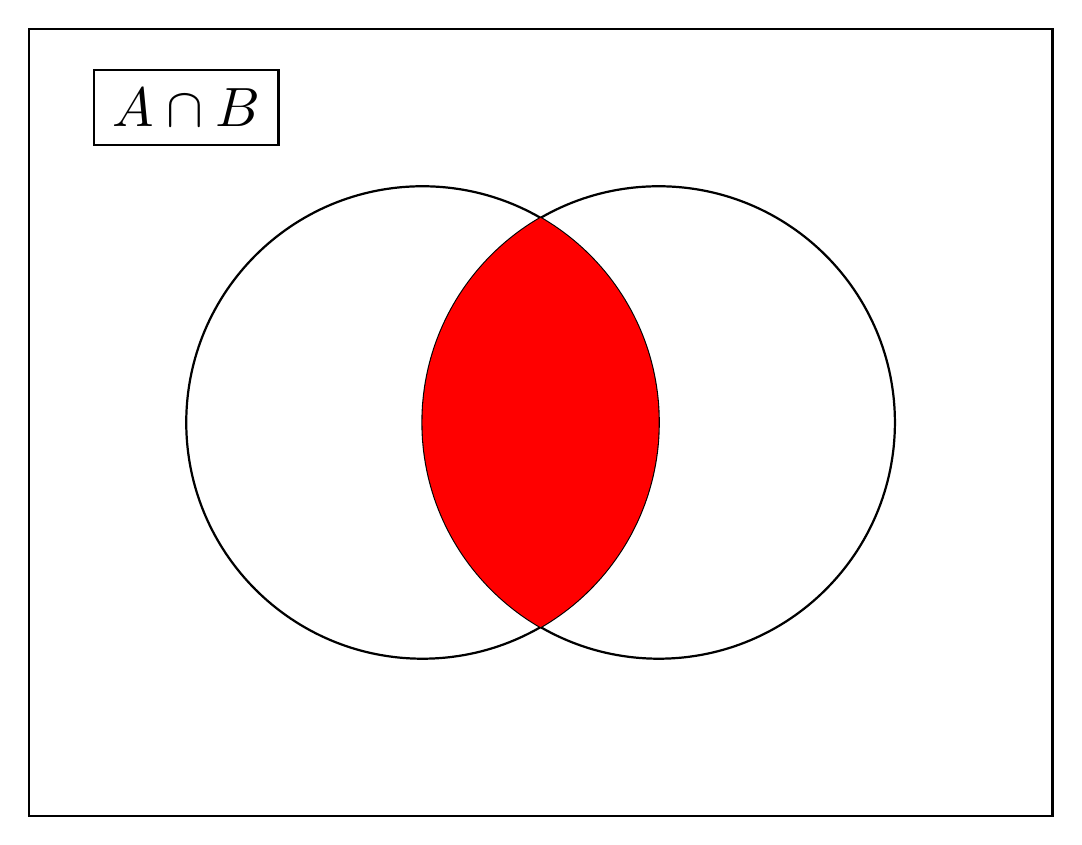
\begin{tikzpicture}[thick,scale=1, every node/.style={scale=2}]

% draw the space
\filldraw[fill=white] (-5,-5) rectangle (8,5);

% the circles
\draw (0,0) circle (3);
\draw (3,0) circle (3);

% A \cap B
\scope 
\clip (0,0) circle (3);
\fill[red] (3,0) circle (3);
\endscope

\node[draw] at (-3,4) {$A \cap B$};

\end{tikzpicture}
\end{document}
